\chapter{Aprendizagem de Máquina}
Como Bishop \cite{bishop2006pattern} descreve, aprendizagem de máquina é uma maneira de abordar um problema de computação. Nessa abordagem, a partir de um grande conjunto de dados, chamados como conjunto de treinamento, são inferidos um conjunto de parâmetros que a serem utilizados em um modelo parametrizado.

\section{Definições}

Algumas breves definições serão apresentadas para fim de ambientar o leitor nos temas discutidos neste capítulo.

\subsection{Amostra}
Seja amostra o conjunto de exemplos que representam os dados conhecidos do problema.

\subsection{Características}
Sejam características um conjunto ordenado de valores que descrevem um exemplo, a ser modelada pelo algoritmo de Aprendizagem.

\subsection{Etiquetas}
Seja etiqueta de exemplo, ou simplesmente etiqueta, a saída esperada do modelo para aquela instância.

\subsection{Avaliações de Desempenho}
Define-se acurácia como:
\[\frac{\mathrm{\#Acertos}}{\mathrm{\#Amostra}}\]

Define-se precisão como:
\[\frac{\mathrm{Verdadeiros Positivos}}{\mathrm{\#Positivos}}\]

Define-se \textit{recall} como:
\[\frac{\mathrm{Verdadeiros Positivos}}{\mathrm{\#Acertos}}\]

Define-se \textit{F1 score} como:
\[\frac{2 * \mathrm{precisão} * \mathrm{recall}}{\mathrm{precisão} + \mathrm{recall}}\]

\subsection{Matriz \(\mathbf{X}\)}
Seja \(\mathbf{X}\), amostra de treinamento, uma matriz \(m \times n\), o qual \(m\) é quantidade de instâncias e \(n\) é a quantidade de características. \(\mathbf{X}\) é a representação matemática da amostra.

\subsection{Vetor \(\mathbf{Y}\)}
Seja \(\mathbf{Y}\), conjunto de etiquetas, um vetor de tamanho \(m\), a quantidade de instâncias, \(\mathbf{Y}\) é o conjunto ordenado das respectivas saídas esperadas de cada linha da matriz \(\mathbf{X}\), ou seja as etiquetas.


\section{Categorias de Problemas}

Para ser mais específico, é possível classificar os problemas resolvidos pela aprendizagem de máquina em cinco categorias\cite{mohri2012foundations}.

\begin{description}
\item \textbf{Classificação}: Decidir a classe de exemplo dadas as suas características, por exemplo decidir qual dígito foi escrito a apartir de uma imagem de dígito escrita a mão.
\item \textbf{Regressão}: Determinar um valor real para cada exemplo, por exemplo o risco de um paciente ter contraído câncer a partir de imagens e resultados de exames.
\item \textbf{Graduação}: Ordenar os exemplos a partir de algum critério, por exemplo listar produtos por relevância a partir das palavras chaves da busca do usuário.
\item \textbf{Aglutinação}: Particionar os exemplos em regiões homogêneas, por exemplo identificar comunidades dentro de redes sociais massivas.
\item \textbf{Redução de Dimensionalidade}: Representar a amostra com número reduzido de dimensões, por exemplo comprimindo imagens para processamento de imagens.
\end{description}

Neste projeto foi decidido encarar o problema como aglutinação, apesar de também poder se confundir com classificação, já que o objetivo é auxiliar a detecção de botnets.

\section{Cenários dos Dados}

Categoriza-se\cite{mohri2012foundations} sete cenários para os algoritmos de aprendizagem, esse cenários são fortemente influenciados pelas condições dos dados de treinamento.

\begin{description}
\item \textbf{Aprendizado Supervisionado}: O modelo tem acesso a dados com e resultados de saída já esperados, ou etiquetados, como lê-se na literatura. Os problemas mais comuns desse tipo de cenários são classificação, regressão e graduação.

\item \textbf{Aprendizado Não Supervisionado}: Só se dispõe da amostra de treinamento sem etiquetas. Geralmente é mais utilizado para classificação, aglutinação e redução de dimensionalidade

\item \textbf{Aprendizado Semi-Supervisionado}: Neste cenário, é possível acessar uma amostra sem etiquetas e uma com etiquetas. Esse é o caso de problemas em que dados sem etiquetas são fáceis de serem adiquiridos, ao contrário dos dados etiquetados, pela dificuldade de etiquetar.

\item \textbf{Inferência Transdutiva}: Semelhante ao Aprendizado Semi-Supervisionado, nem todos os exemplos são etiquetados, mas o modelo só deve ser generalizado apenas para os exemplos conhecidos.

\item \textbf{Aprendizado On-line}: Neste cenário, iterasse no modelo a cada exemplo recebido em rodadas. No início da rodada, o modelo recebe um exemplo, inicialmente sem etiqueta, realiza uma predição, recebe a etiqueta e atualiza os parâmetros do modelo.

\item \textbf{Aprendizado por Reforço}: Neste cenário, os modelos são criados baseado num sistema de recompensa. O modelo é recompensado a cada decisão bem feita ao interagir com um ambiente.

\item \textbf{Aprendizado Ativo}: O algoritmo é quem realiza requisições a uma entidade capaz de etiquetar exemplos para melhorar os parâmetros do modelo. O objetivo é conseguir gerar um modelo tão bom quando o modelo supervisionado, porém com menos exemplos.

\end{description}

E ainda há outras possíveis cenários ainda mais complexos e específicos, não catalogados neste trabalho porque a ciência de Aprendizado de Máquina está ainda em constante fase de crescimento.

\section{Exemplo: Regressão Supervisionada}

Dado um conjunto de tamanho de imóveis e seus respectivos valores de compra em uma vizinhança hipotética estimar o valor de um apartamento sabendo apenas seu tamanho.

Seja o vetor ordenado \(\mathbf{X} = [x_{1},x_{2},...,x_{m}]\), \(\#\mathbf{X} = m\), o tamanho em Metros quadrados de apartamentos em um bairro. Seja \(\mathbf{Y} = [y_{1},y_{2},...,y_{m}]\), o preço do i-ésimo apartamento indexado em \(\mathbf{X}\). Se arranjarmos os valores graficamente obtem-se a Figura 1.

\begin{figure}
	\centering
		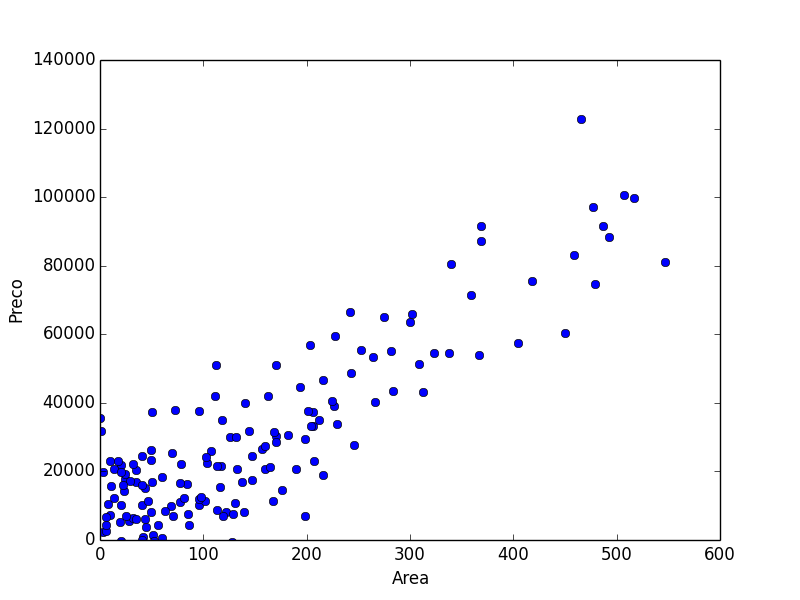
\includegraphics[width=0.9\textwidth]{figure_1.png}
		\caption{a distribuição do preço das casas}
		\label{casas}
\end{figure}

Suponha que de posse do tamanho \(x\), não apresentado em \(\mathbf{X}\), o usuário queira inferir um preço \(y\). Para tal é necessário construir uma hipotese \(h_{\theta}\) que melhor interpole os valores de já conhecidos. Para poder avaliar se \(h_{\theta}\) é ótimo, existe uma função custo, \(custo(h_{\theta},\mathbf{Y})\).

Para esse problema, considera-se:

\[h_{\theta}(x) = \theta_{1}*x + \theta_{0}\]

Ou seja, um modelo linear. Além disso, para avaliar a proximidade do modelo e da amostra, aplica-se o erro quadrádico médio como função custo, isto é:

\[custo(h_{\theta}(X),\mathbf{Y}) = \frac{1}{m}*\sum_{i=1}^{m}(h(x_{i})-y_{i})^2\]

Tem-se dados, função de custo, precisa-se introduzir um método de otimização. Propõe-se, então, o uso Método do Gradiente, que é um método para achar o mínimo local dado um ponto. Como a função de custo em questão é quadrática, ou seja, é convexa. Existe \(\alpha\) tal que atualizando iterativamente os parâmetros \(\theta_{0}\) e \(\theta_{1}\), seguindo a expressão

\[\theta_{0} = \theta_{0} - \alpha * \frac{\partial}{\partial \theta_{0}}  custo(h_{\theta}(X),Y)\]
\[\theta_{1} = \theta_{1} - \alpha * \frac{\partial}{\partial \theta_{1}}  custo(h_{\theta}(X),Y)\]

Converge-se à solução ótima que minimiza o valor da função custo, sendo possível com algum erro inferir o valor do imóvel sabendo seu tamanho. Tal hipótese \(h_{\theta}\) está representado na Figura 2

\begin{figure}
	\centering
		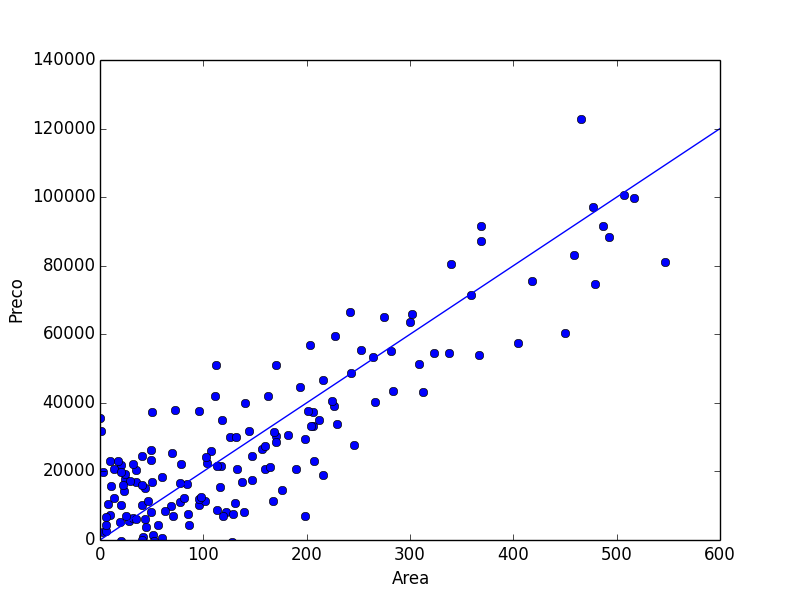
\includegraphics[width=0.9\textwidth]{figure_2.png}
		\caption{o modelo acompanhado e a distribuição do preço das casas}
		\label{casas}
\end{figure}



\section{Detecção de Anomalia}

O artigo, \textit{Anomaly Detection: A Survey}\cite{chandola2009anomaly}, define Detecção de Anomalia o problema da busca por padrões nos dados que não seguem um padrão de um comportamento esperado. Essas anomalias podem acontecer em diversos contextos, ruídos nas medidas, defeitos em equipamentos, comportamentos inovadores ou até atividades fraudulentas, como fraude de cartão de crédito e ataques cibernéticos. Esse tipo de algoritmo pode ser utilizado para resolver problemas de Classificação e Aglutinação.

\subsection{Etiquetas em Detecção de Anomalia}

Geralmente a tarefa etiquetar os dados de modo representativo e preciso é custosa. A forma mais comum de etiquetagem é feita manualmente por um especialista. Esse processo é geralmente custoso, pois são necessários muitos exemplos para encontrar uma anomalia, que por definição é um caso raro. Dentro desse contexto, existem 3 cenários possíveis na operação da Detecção de Anomalias, Supervisionado, Semi-Supervisionado, Não Supervisionado.

Os algoritmos de Detecção de Anomalia Supervisionados convertem têm poucos exemplos de anomalias, por definição, que isso pode trazer problemas quanto a análise da acurácia. O caso extremo seria considerar todos normais e ter acurácia de alta, uma vez que os exemplos anomalos podem representar menos de \(1\%\) da amostra. Isso pode ser resolvido observando a precisão e a exaustividade que resultariam \(0\%\). Como é preciso se chegar em um número para poder comparar performance, Witten\cite{witten2011data} propõe que se avalie o \textit{F1 score}, que seria a média harmônica das duas medidas.

Assume-se que as amostras de treinamento são exemplos etiquetados como normais quando se trabalha no cenário Semi-Supervisionados desse modo é possível criar uma estimativa de como se comportam os exemplos normais e assumir que os que fogem do escopo é anomalia.

Por último, quando não se tem etiqueta para os exemplos opera-se num cenário Não Supervisionado, assume-se que os casos anoma-los são menos frequentes. Note que se essa premissa não for satisfeita, o sistema está sujeito à alta quantidade falsos negativos.

\subsection{Proposta de Modelo}

Será exposto um modelo de Detecção de Anomalia baseado em modelo probabilístico. Suponha que os dados de uma determinada amostra se distribuam no plano determinado pelas características de acordo com o padrão normal. Dessa forma é possível associar cada exemplo \(\mathbf{x}\) à uma probabilidade, \(p(\mathbf{x})\).
Sabe-se\cite{bishop2006pattern} que a distribuição normal multidimensional é

\[\mathcal{N}(\mathbf{x}|\mathbf{\mu},\mathbf{\Sigma})=\frac{1}{(2\pi)^{\sfrac{D}{2}}} \frac{1}{|\mathbf{\Sigma}|^{\sfrac{1}{2}}}\exp\left\{ -\frac{1}{2} (\mathbf{x} - \mathbf{\mu})^T \mathbf{\Sigma}^{-1} (\mathbf{x} - \mathbf{\mu}) \right\}\]

O qual \(D\) é a dimenção de \(\mathbf{x}\), \(\mathbf{\mu}\) é o vetor média de todas as caracteríticas da Matriz \(\mathbf{X}\) e \(\mathbf{\Sigma}\) é uma matriz covariância, \(D \times D\), \(|\mathbf{\Sigma}|\) é seu determinante.

\[\mathbf{\Sigma}=\mathit{cov}[ \mathbf{x} ] = \mathbb{E} \left \lbrack ( \mathbf{x} - \mathbb{E} [ \mathbf{x} ] ) ( x - \mathbb{E} [ \mathbf{x} ] ) ^ T \right \rbrack \]

O qual \(\mathbb{E}\) é o operador valor esperado. Após a construção do modelo probabilístico, o algoritmo decide se tal um novo exemplo \(\mathbf{x}\) é uma anomalia se

\[\mathcal{N}(\mathbf{x}|\mathbf{\mu},\mathbf{\Sigma}) < \varepsilon\]

O qual \(\varepsilon\) é um valor gatilho escolhido previamente que resultou, por exemplo o melhor \textit{F1 score}, se o modelo for aplicado em um cenário Supervisionado.
